\subsection{Layout and structuring}
As mentioned in Chapter \ref{motivations}, one of the main problems I had with ARM programming was keeping my code organised as I was learning the intricacies of ARM while trying to write code. Now armed with a little more experience, I wanted to ensure that my code was kept organised from the start. I decided the best way to start would be to organise my main file \verb|os.s|. It had a lot of the handlers required in the same file, which I felt was not great practice as it does not allow for a separation of concerns. I organised this file by making use of the INCLUDE mnemonic. This mnemonic is similar in concept to an import command in Java or Python except it differs in its exact implementation. The INCLUDE directive provided by my assembler has the effect of moving the code from the specified file to the location of the INCLUDE command. This is close to how C implements include. % reference here?

\begin{lstlisting}[
	style = myListingStyle,
	caption = {My main os.s file}
]
	ORIGIN &00000000
	B hard_reset                          ; +0   (00)
	B undefined_instruction_handler       ; +4   (04)
	B svc_handler                         ; +8   (08)
	B prefetch_abort_handler              ; +12  (0C)
	B data_abort_handler                  ; +16  (10)
	NOP                                   ; +20  (14)
	B IRQ_handler                         ; +24  (18)
	B FIQ_handler                         ; +28  (1C)

	halt ; should be jumped to, to stop the proccessor
	MOV R0, R0
	B halt

	; Import handlers
	INCLUDE handlers/reset_handler.s
	INCLUDE handlers/instruction_handler.s
 		...

	; Import definitions
	INCLUDE general/printchar.s
	INCLUDE general/printstring.s
  		...

	ALIGN
	INCLUDE general/usercode.s

\end{lstlisting}


My \verb|os.s| file also included a halt loop which I could jump to as a way of `halting` the processor as there is no way for the processor to halt itself
This really helped with debugging as I could use this loop to stop the processor after an error without it changing the state of any memory addresses. An issue I had encountered a lot in past course was that when I would run into something like a data abort or an undefined instruction, I would have nothing to stop the processor from overrunning the handler it would jump to. This would quite often make things hard to debug. Having the halt instruction allowed me to give the processor some control over halting itself.
\subsection{Self Imposed Conventions}
To keep my code organised and readable, I picked up a few conventions along the way which I tried to stick to. These were chosen with the intention of making my code easier to update in the long run as ARM is a difficult language to read. One of the conventions I stuck to best was to comment every procedure call under the label with a definition of which registers are used for input and output. This format provided me with an easy way to look up my method's and determine how to use them. Another benefit of this format is it distinguishes the branch label from other labels as an actual procedure call. Another convention I employed was the consistent pushing style of registers. When a procedure starts I always immediately push the LR, regardless of whether I need to. This is so that if I require a call to another procedure call, I don't need to remember to push the LR as it is already done. If I hadn't done this, then each time I needed to add a nested procedure call, if I forgot to push the LR then I would have an error on my hands which I would likely have to hand trace to debug. Similarly, when writing a new procedure, I would also push the registers I need to work in, and then immediately pop them, and then write the procedure in between. This meant that I could more closely mimic writing in a higher level language as I didn't have to think as much about the unusual parts of ARM. An example of these conventions is described below
\begin{lstlisting}[
	style = myListingStyle,
	caption = {How all of the procedure calls started}
	]
	queue_index
	; IN  R0 - index to check
	; IN  R1 - Pointer to queue
	; OUT R2 - item to return or -1 if invalid
	PUSH {R0 - R1, R3 - R12, LR}
	
	; Actual procedure code goes here.	
	
	PUSH {R0 - R1, R3 - R12, PC}  ;return
	
\end{lstlisting}
I also utilised the \verb|EQU| directive often, in order to aid the readability of my code. For any constant or immediate value used (other than simple values such as -1, 0, 1, 2, 4) I would aim to name them, and then only use the label. Another benefit of using this directive is that I could use them to do arithmetic to define how much space I would statically assign to blocks of memory. This was useful when designing the process control block, as I could scale how much memory I would need according to a single constant MAX\_THREADS. The ability to perform arithmetic operations with aliased names made scaling the program much easier. 
Finally, the last convention I imposed on myself was to write a commentary along some of the more technically challenging aspects of the code. For example the context switching procedure is the most complex thing I've written in ARM if not in all languages. So while writing this code I would start by writing a short comment describing the small subtask I wanted to complete, before  writing the code to complete this subtask. This was quite a time-consuming process, as any changes which I needed to make usually meant that I had to re-write my comments. Due to this, I only employed this strategy when it was really necessary. I found this so helpful, that I would often describe the problems I needed to overcome for a specific subroutine in the subroutines' header. This acted as a cheaper way of documenting my code well without spending too much time on it. 
\subsection{Virtual Screen}
The installation of Komodo which I was developing for had a virtual screen (as described in figure \ref{fig:LCDMem}) which I could manipulate. I wanted to provide some methods to the user which could be used to manipulate the screen. The screen appears in memory as a large frame buffer. This is in contrast to how most real world alternatives would present themselves. For example, if you were to use a Hitachi HD44780 \cite{datasheet}, you would find that it presents its self as a more `intelligent` controllable device. Rather than writing directly to the frame-buffer to write characters, it is far more efficient to give it commands to write the characters, which it can then carry out itself. As the virtual screen does not contain these methods, I have to make them myself. I have done this before, however I felt I had an opportunity to improve upon this code. My previous code also could only print in black and white which I felt was somewhere I could improve in. My new functions would take a pointer to a string as a parameter as well as a pointer to 6 bytes defining the RGB colour of the background and text colour. 


The procedure I developed to print a single character is shown in listing \ref{lst:printchar_pseudo}. This procedure would be called for every character in a string in order to provide the print string function. 
\begin{lstlisting}[
	style = myListingStyle,
	caption = {printchar pseudocode},
	label={lst:printchar_pseudo}	
	]
	if ( char is a control character ) {	
		update cursorposx according to char
		correct to ensure 0 <= cursorposx <= 40
		update cursorposy according to char
		correct to ensure 0 <= cursorposy <= 30
	} else if ( char is a letter ) {
		print the character
		update cursorposx
		update cursorposy
	} else {
		halt the processor
	}
\end{lstlisting}
The challenge of writing characters to the screen essentially boils down to two main problems - Outputting a character template and keeping track of where the cursor is. Both problems are relatively trivial to solve, however how to write code to solve them efficiently is difficult.
\subsubsection{Keeping the cursor position consistent}
I solved this problem by first handling the control characters. These characters are the ASCII characters used to control the movement of the cursor. I chose to determine which control character I was working with via a simple jump table. This has the benefit of allowing me to add more control characters easily. Once I have jumped to the correct position I can then perform the correct operation. From here I then update the cursor position by performing the update and then checking and correcting the x and y coordinate against the bounds of the screen. A similar method is employed to correct the cursor after writing a character. Essentially every operation on the screen should leave the cursor in a position ready to print a new character. The characters I have supported are listed, and their effect is seen in Table \ref{controlcharacters}.
\begin{table}[H]
	\centering
	\caption{Supported control characters.\label{controlcharacters}}
	\begin{tabular}{|c|c|}
		\hline
		Backspace & Delete a character left of the cursor \\
		Horizontal Tab & Move the cursor right \\
		Line Feed & Move the cursor down one line \\
		Vertical Tab & Move the cursor up one line \\
		Form feed & Clear the screen \\
		Carriage return & Move the cursor to the start of the next line \\
		\hline
	\end{tabular}
\end{table}
\subsubsection{Outputting a character}
To output a character I use a 7 x 8 pixel font. It provides a font for ASCII characters 32 to 126. To determine the address of the font I have to subtract 32 from the character to normalise the character to the base of my font map. I then multiply by 7 bytes to determine the correct address. From here I have to read the loop over the 7 bytes as a 2d array essentially, with one dimension as the bytes and one dimension as the bits as demonstrated in figure \ref{fig:fontexample}.


\begin{figure}[H]
	\begin{subfigure}{0.5\linewidth}
		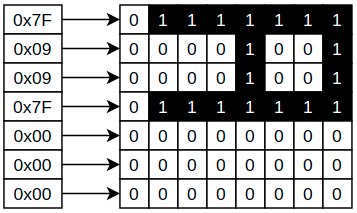
\includegraphics[width=\linewidth]{figures/font.png}
	\end{subfigure}
	\begin{subfigure}{0.5\linewidth}
		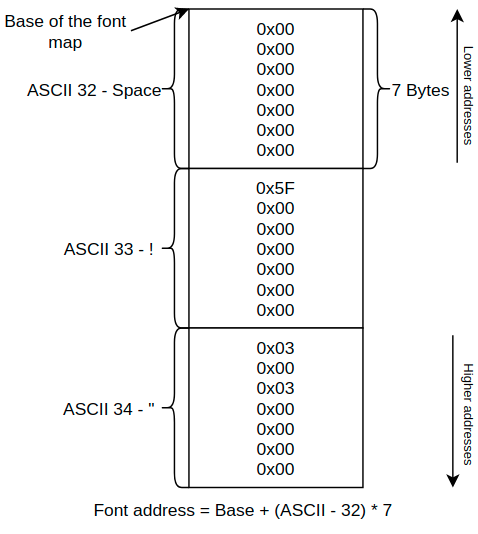
\includegraphics[width=\linewidth]{figures/fontmap.png}
	\end{subfigure}
	

	\caption{The font set-up in memory}
	\label{fig:fontexample}
\end{figure} 




\subsection{The SVC Handler}
The SVC handler is a program used to allow users to safely execute code which may require higher privileges. For example, if a user wanted to read data from a peripheral, this may be acceptable to the OS, but it has to be done in a controlled way. The OS provides the SVC handler as a way of enabling this access without letting the user handle the specifics. The handler provides an organised way to interpret an SVC instruction and determine which operation to direct the processor to. It determines which program to jump to by reading the instruction in the link register. The handler will read the instruction pointed to by the LR and strip the instruction of its op code. This has the effect of leaving the parameter of the SVC instruction which can be used to compare against the implemented SVC routines. It checks this code against the SVC\_MAX constant. This constant defines the highest identifier supported by the chip.  This is a security measure to ensure that the SVC command cannot branch to any arbitrary code. In a single ADD instruction it then multiplies the SVC constant by 4 to get a words address and then adds it to the PC. The next instruction loads the address at this address to the program counter which causes the handler to jump to the correct position. This jump table method is also described in listing \ref{lst:svcexample}. I chose the jump table method as I needed to support 12 methods, so a long chain of switch statements to determine the SVC parameter would not be particularly efficient. The jump table method is a far more effective way of directing execution to the correct procedure


\begin{lstlisting}[
	style = myListingStyle,
	caption = {The SVC handler},
	label = {lst:svcexample}
	]
	LDR R14, [LR, #-4]        ; Read the caller svc command into R14
	BIC R14, R14, #&FF000000  ; Clear the opcode
	
	LDR R3, SVC_MAX	          ; Check user is not trying to execute arbitrary code
	CMP R14, R3 
	BHI SVC_unknown
	
	SUB R14, R14, #&100       ; Normalise base of SVCs
	ADD R14, PC, R14, LSL #2  ; Calculate SVC jump point in the table
	LDR PC, [R14] 		  ; Perform Jump       
	
	DEFW SVC_0  ; halt
	DEFW SVC_1  ; printchar
	DEFW SVC_2  ; printstr
	...	
	
\end{lstlisting}


The operations I supported are as follows:

\begin{tabular}{cl cl}
	halt & (Halts the processor) \\
	printchar & (Prints a character to the virtual LCD) \\
	printstring & (Prints a NUL terminated string to the virtual LCD) \\
	timer & (Copies the timer into R0) \\
	button data  & (Gets the data from the virtual buttons \textit{deprecated}) \\
	setcursorposx & (Sets the horizontal position of the cursor) \\
	setcursorposy & (Sets the vertical position of the cursor) \\
	query\_keyboard & (Grabs the first pushed key from the virtual keyboard) \\
	query\_key & (Checks if a specific key is pushed) \\
	create\_thread & (Starts a thread from a specified address) \\
	end\_thread & (Kills the current thread) \\
	halt\_thread\_for\_IO & (Halts the thread until input occurs and then runs query\_keyboard) \\
\end{tabular} 
\bigskip

My SVC handler also includes a brief exit procedure which is always jumped to after completing an operation. This procedure just re-enables interrupts as the processor disables them during the SVC entry procedure to ensure that the operations execute atomically. 
%\subsection{The IRQ Handler}
\subsection{The Reset Handler}
The system should be able to run from two different but similar starting points. The usual way to run the code is to load the assemble files into Komodo and run them. However, Komodo also provides a reset function button. This button has the following effect:

\begin{lstlisting}[
	style = myListingStyle,
	caption = {The reset mechanic provided by ARM},
	label = {lst:reset}
	]
	PC <= 0x0000_0000
	Mode <= Supervisor
	Interrupts <= Disabled
\end{lstlisting}
The reset function means that I have to reset enough of my state in my reset handler in order to create a recoverable state. Without careful and consistent updates to my reset handler, I can run into a situation where a reset does not correctly reset read/write data statically defined in memory. Take for example the \verb|cursorposx| and \verb|cursorposy| memory locations. These represent the coordinates of the next character on the screen to be written to. Reloading the assembled code in Komodo will correctly set these values to 0,0 respectively. However, if the reset button is pushed, these addresses must be written to in order to reset them. Some of the actions my reset handler must perform are as follows:

\begin{itemize}
	\item Move the cursor back to 0,0
	\item Clear the screen
	\item Reset the timer
	\item Reinitialise the pointers of the SVC and IRQ stacks
	\item Clear the PCB of previous processes
	\item Re-enable interrupts
	\item Initialise the main thread
\end{itemize}

Thankfully, this task is simplified by most of the memory being assumed to be undefined. This means that data structures like the stack, I can merely reset the pointer, and future memory will be overwritten during execution.

\begin{figure}[ht!]
	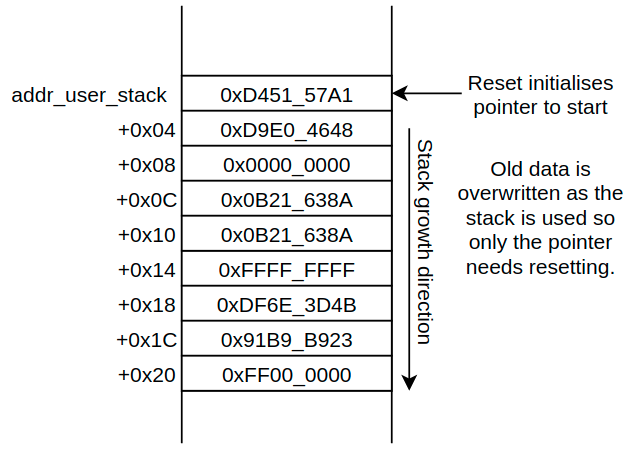
\includegraphics[width=\linewidth]{figures/reset.png}
	\caption{How stacks are reset.}
	\label{fig:reset}
\end{figure} 


\subsection{Data Structures and Unit testing}
When writing in assembly, the lack of features can be an issue in need of resolving. For example, in a high level language like python for example, you can create a list in memory by a single command: 


\begin{lstlisting}[
	style = myListingStyle,
	label = {lst:pythonlist}
	]
	my_list = []
\end{lstlisting}

In python this gives you access to various operation you can perform on the list such as \verb|append()|, \verb|insert|, \verb|pop()|, \verb|len()| and  \verb|sort()| to name a few. In contrast, in ARM the equivalent code would have to be written and tested by yourself. Therefore, as I knew I would need a queue data structure to implement the scheduler, I developed an implementation for a queue, with procedures I could call,
 such as \verb|queue_push|, \verb|queue_pop|, \verb|queue_utilisation|, \verb|clear_queue|, \verb|queue_find| and \verb|queue_index|. In my experience data structures like these usually form the building blocks of code, so they have to be well tested, so you can rely on their operation. Hence, I decided to experiment with unit testing in ARM. In previous work in higher level languages, I have used technologies such as JUnit \cite{junit} and Nunit \cite{nunit} to test Java \cite{java} and C\# \cite{csharp} code respectively.  I wanted to test my code in a similar style, using unit tests to test individual procedure calls and test their functionality. This was with the ultimate goal of developing a data structure which had been properly debugged before its use. I developed the files \verb|queue.s| and \verb|queue_testing.s| which contained the implementation of a queue and the unit test for this data structure respectively. I found that creating a testing suite for pivotal blocks of code like this was a particularly effective way of ensuring the reliability of critical code. Throughout the remainder of the project, I did not encounter any bugs regarding my queue implementation. 






















